
%%%%%%%%%%%%%%%%%%%%%%% file typeinst.tex %%%%%%%%%%%%%%%%%%%%%%%%%
%
% This is the LaTeX source for the instructions to authors using
% the LaTeX document class 'llncs.cls' for contributions to
% the Lecture Notes in Computer Sciences series.
% http://www.springer.com/lncs       Springer Heidelberg 2006/05/04
%
% It may be used as a template for your own input - copy it
% to a new file with a new name and use it as the basis
% for your article.
%
% NB: the document class 'llncs' has its own and detailed documentation, see
% ftp://ftp.springer.de/data/pubftp/pub/tex/latex/llncs/latex2e/llncsdoc.pdf
%
%%%%%%%%%%%%%%%%%%%%%%%%%%%%%%%%%%%%%%%%%%%%%%%%%%%%%%%%%%%%%%%%%%%


\documentclass[runningheads,a4paper]{llncs}

\usepackage{amssymb}
\setcounter{tocdepth}{3}
\usepackage{graphicx}

\usepackage{url}
\urldef{\mailsa}\path|{m.martineau,cssnmis}@bristol.ac.uk|    
\newcommand{\keywords}[1]{\par\addvspace\baselineskip
\noindent\keywordname\enspace\ignorespaces#1}

\begin{document}

\mainmatter  % start of an individual contribution

% first the title is needed
\title{On the Dominance of Performance Characteristics in Highly Parallel HPC Packages}

% a short form should be given in case it is too long for the running head
\titlerunning{Composing the Dwarfs}

\author{Matt Martineau \and Simon McIntosh-Smith}
%
\authorrunning{Composing the Dwarfs}

% the affiliations are given next; don't give your e-mail address
% unless you accept that it will be published
\institute{Merchant Venturers Building, Woodland Road, Bristol, BS82AA, United Kingdom\\
  \mailsa\\
\url{}}

%
% NB: a more complex sample for affiliations and the mapping to the
% corresponding authors can be found in the file "llncs.dem"
% (search for the string "\mainmatter" where a contribution starts).
% "llncs.dem" accompanies the document class "llncs.cls".
%

%\toctitle{Lecture Notes in Computer Science}
%\tocauthor{Authors' Instructions}
\maketitle


\begin{abstract}
  In this paper we discuss the composition of parallel packages, and how this affects performance on highly parallel supercomputing hardware. We introduce four new mini-apps, Fast, Hot, Wet, and Bright, which perform a parallel FFT, solve heat diffusion and hydrodynamics, and track neutral particles. The mini-apps represent four of the seven Dwarfs of parallel programming, and have been developed with the purpose of evaluating the impact of coupling those algorithms together.

  Although much research has been performed that evaluates the performance profile of the seven Dwargs, production applications rarely utilise only a single package in solving a scientific problem. We present a motivational comparison of the Dwarfs, considering the theoretical impact of coupling them together. Following this we present performance results of coupling several new mini-apps together and using them to solve test problems on modern hardware including Intel Xeon Broadwell, Xeon Phi, IBM Power8, NVIDIA Kepler, and NVIDIA Pascal.

\keywords{performance portability,mini-apps,high performance computing,openmp 4}
\end{abstract}

Modern supercomputing has reached a scale where the core counts at the node level are increasingly significantly each year, and this has major implications for writing portable and performant code. In particular, many of the largest supercomputers in the world include heterogeneous devices, such as accelerators, which greatly increase the core count, and require that significant data-parallelism is exposed within scientific application's algorithms in order to perform well.

Accelerator devices like the Intel Xeon Phi processors, have greater numbers of cores than existing Intel CPUs, for instance the Knights Landing has between 64 and 72, each with 4 hardware threads, whereas the Intel Xeon Broadwell can have up to 22 cores per socket, with less chance that the 2 available hyperthreads will help performance for HPC applications. The IBM POWER8 CPU also exposes a large core count, with up to 12 cores per socket and 8 hardware threads for a total of 192 (DOUBLE CHECK THIS) threads in total.

Extending the discussion to GPGPUs, NVIDIA's Tesla K40 devices have 15 streaming multi-processors (SMX), each of which support 192 processing elements, for a total of 2880 CUDA cores. While those cores aren't not cores in the traditional sense, given that instructions are issued to warps which operate in lock-step, it is clear that a great deal of parallelism needs to be exposed in order to target them. More recently, NVIDIA released the Tesla P100, which has increased the number of SMXs to 56 and decreased the number of processing elements in each to 64 (two warps), for a total of 3584 CUDA cores in total.

Of course, this continual increase in the number of cores available on a node has major implications for the scalability of codes, and this is amplified by the increasing number of nodes that are hosting those devices. 

Our previous work has shown that there are issues with scaling many scientific applications past a certain point, regardless of their node-level performance, as communication becomes the limiting factor. It would appear that we are reaching a stage where the scalability of applications demands that the highly parallel nodes are programmed using shared memory programming, in order to reduce the number of independent ranks that need communication. 

The benefit of GPUs is that they offer good performance and can handle significant portions of a problem and require no partitioning within the devices. More recently supercomputing resources have started to include multiple accelerator devices on a single node, and this offers the opportunity for programmers to exploit massive node-level parallelism to improve the scalability of applications. Of course this requires that there is some suitably performant method for communicating within a node. The upcoming NVLINK technology that will be distributed by NVIDIA is intended to provide fast communications between the GPUs on a node and quite improved performance compared to PCIe when communicating with the host CPU. Our expectation is that if this technology can be used to its full extent, it should offer great potential improvements to the scalability of HPC applications. 

It is considered an onerous and complicated task to program GPUs and until recently there has been little traction within the community to port existing large-scale applications, even though some of the largest supercomputers in the world, for instance Titan, include both CPUs and GPUs. We have shown in our previous research that GPUs can be programmed effectively, in most cases, using existing programming models. We have shown that productivity can be an important deciding factor in the choice of programming model, and further showed that directive-based models can offer a highly productive interface, that can be portable given good implementations, whilst not significantly sacrificing performance.

Many of our findings and discussions have been limited to individual applications which have, in general, performed well on modern hardware, and with modern parallel programming models. However, they do not represent that true form of large-scale scientific applications, in that they are isolated instances of algorithms that have do not represent the multi-application hierarchies that scientists are truly interested in seeing results for.

Our intention is to use a new suite of mini-apps, tailored for composition, to expose the dominantn performance characteristics when combining multiple applications as would be seen in a common scientific production application. We have attempted to make the mini-apps general, but have been careful to ensure that they capture the desired performance profiles of their proxied applications.

\section{Contributions}

As part of this research and throughout this paper we present a number of contributions:

\begin{itemize}
    \item We have developed three new mini-apps that serve as proxy applications for important scientific algorithms. A heat conduction application, a fluid dynamics application, and a Monte Carlo Particle Transport application.

\item We demonstrate our approach to coupling those applications, both physically and in terms of the computer science aspects including mesh decomposition strategies.

\item We present results for those algorithms in isolation on modern supercomputing devices: a NVIDIA Tesla P100, an Intel Xeon Phi Knights Landing processor, an IBM POWER8 CPU, and a Intel Xeon Broadwell.

  \item We present the results of running those applications at scale, on those same devices.

    \item We present early results for running the Hot and Wet mini-apps coupled together into a single multi-package application.
\end{itemize}

\section{Background}

In this section we will present some basic details about each application, in order to make clear what each application is intended to simulate. Our intention was to choose the simplest methods possible, whilst achieving a reasonable level of accuracy, and in particuler focused upon capturing the performance profile of their respective classes of algorithms.

In order to give a clear discussion, we will explain the initial development of each application prior to discussing our efforts to couple them together. This means that we will explain how each application was optimally developed, but with the caveat that this would likely have to change once coupling was required. We did not particularly consider the coupling up-front, instead opting to choose the best strategy for each application in isolation, maximising the potential outcomes of the coupling exercise.

\subsection{Composition of Dwarfs}

When considering the coupling of parallel algorithms, there is the potential to consider any number of existing packages. In this research we have chosen to continue on from the work discussed by Asanovic et al. \cite{Asanovic2006}, who outlined a number of Dwarfs, each of which describes a different computational class that features in modern supercomputing applications. They continue to describe an additional 6 Dwarfs, but this paper will only investigate the original seven.

Each of the Dwarfs has a unique set of computational and communicational characteristics that mean that they have different requirements of modern computing hardware. While many of those characteristics have been analysed and optimised heavily on existing architectures, we hope to uncover the extent to which those classes can co-exist within an application. At this stage we will re-iterate that that the majority of production applications that solve significant scientific problems will require packages encompassing a number of the classes described by the Dwarfs.

The classes described by the Dwarfs are broad, and they encapsulate a subset of possible performance characteristics, which may be present in other Dwarfs. We hope to discover which is of those characteristics is most important, in the context of parallel performance on modern hardware, by considering the Structured Grid, Monte Carlo, Sparse Linear Algebra, and Spectral Methods Dwarfs. In particular, we consider four applications of those classes, hydrodynamics (Wet), neutral particle tracking (Bright), implicit heat diffusion (Hot), and the Fast Fourier Transform (Fast).

Some of the most important performance characteristics of those particular applications are listed in Table \ref{tab:perf-char-mini-apps}.

\begin{table}[h]
  \begin{center}
    \begin{tabular}{cccccc}
      \hline
      \textbf{Property} & \textbf{Hot} & \textbf{Wet} & \textbf{Fast} & \textbf{Bright} \\
      \hline
      \textit{\textbf{Nearest Neighbour}} & Yes & Yes & No & No \\
      \textit{\textbf{Dynamic Locality}} & No & No & No & Yes \\
      \textit{\textbf{Inner Iterations}} & Yes & No & No & No \\
      \textit{\textbf{Iterative}} & No & No & No & Yes \\
      \textit{\textbf{Mesh-based}} & Yes & Yes & Yes & Yes \\
    \end{tabular}
  \end{center}
  \caption{Performance characteristics of the four mini-apps.}
  \label{tab:perf-char-mini-apps}
\end{table}

Our intention is to investigate how the computational and communicational profiles of those applications interact with eachother. Prior to discussing the coupling stage and performance evaluations, we will describe the individual applications and how they are developed.



\subsection{Fast}


\subsection{Hot - Heat Conduction via a CG Solver}

We have developed a simple conjugate gradient (CG) solver that implicitly solves the heat conduction equation in order to solve the problem within a reasonable time-frame with acceptable fidelity. Our implementation uses a standard preconditioner, but otherwise adopts the simplest CG approach. 

The conjugate gradient method is iterative, and reduces the error of a guessed solution by walking along the eigenvectors of the solution vector. We will not develop or explain the mathematics underpinning the CG solver, and direct interested readers to explore the wealth of existing literature \cite{} (PUT A LOAD OF CG REFERENCES IN). The only physical feature of the application is manifested in the density calculations, where the densities are stored at the cell centers and interpolated to the edges.

The best decomposition for this algorithm is essentially regular, minimising the surface area to volume of each rank to reduce communication overheads. In terms of boundary conditions we selected reflective, as this was simple, and improves the verifiability of the results. It is also useful when coupling to the other systems.

\subsection{Wet - Fluid Dynamic via Direct Lagrangian-Eulerian Flux Calculations}

Our fluid dynamics simulation maintains the simplest possible methods, whilst keeping second order in space for all dependent variables. We chose to stay first order in time because algorithms that are second-order in time are somewhat more complicated, and the benefit is primarily reduce wallclock time. Our initial instinct is that the relative runtimes of each of the applications was not particularly important at this stage, but may revisit this issue in a later publication.

The direct Lagrangian-Eulerian algorithm takes Euler's equations, and explicitly solves them across a staggered structured grid. The application uses simple smoothing to simulate artificial viscosity, with shock heating accounted for as part of the mechanical work update. For the mass flux calculations, a Van-Leer flux limiter is used to maintain a monotonic profile at shock boundaries, and second-order interpolations are performed for energy and momentum to ensure monotonic behaviour for all dependent variables.

Directional splitting is used in order to make the application two-dimensional, and we chose to maintain symmetry by alternating the directional calculations with each timestep. Our explicit timestep controls limit the timestep based on the artificial viscosity coefficients and stop any flux extending beyond a single cell.

As with the heat condution application, the boundary conditions we chose for this application are reflective. This is particularly useful for fluid dynamics as tracking of conservation is important in verifying the results.

\subsection{Bright - Monte Carlo Particle Transport}

Our transport application uses a Monte Carlo particle tracking method, making it quite different to the other two algorithms. Our initial effort split the problem into batches of particles, each of which had an individual history that was followed in a time-dependent manner. 

A major aspect of the application is the data structure used to describe particles. Given that we did not have prior experience with this particular algorithmic class, we were not exactly sure which of the potential approaches would end up being the most performant, so we explored the space and performed some testing which we describe in detail later. Ultimately, we described a single particle using a data structure that contains the particle's position in space, direction, energy, and initially tracked the particles location by cell on the mesh.

Our simple tracking procedure would maintained several running timesteps to different event types: (1) a Collision event, which is where the particle would either change direction or have some of its weight absorbed, (2) a Facet event, where the particle reached the boundary of a cell or zone, and (3) a Census event, where the particle reached the end of the current timestep. Of course, the census events for the application in isolation were simply set to some small constant size, with the intention for this timestep to be later controlled by the requirement of the CFL condition exposed by the fluid dynamics simulation.

In order to determine if a Collision event has occured, we perform a lookup to cross sectional data taken from the ENDF database. In our particular approximation, we only consider absorption and scattering, ignoring any contributions due to fission. In order to reduce the overall variance of the simulation, we extend the lifespan of particles by giving them a weight, and reducing this weight each time an absorption event occurs, rather than declaring them as dead particles. Once the weight has reduced past a certain point, or the particle has reached a low enough energy, we will only then consider the particle to be dead.

When a Collision event occurs and the result is a scattering of the particle a random number is generated to determine the angle of scattering, and this is also used to determine the level of energy dampening that occurs using well known relations \cite{}.

To perform facet intersection checking, we are able to leverage the simple geometry of the structured grid to calculate the new direction using a simple method of our own devising. We first check which of the edges would be hit first if the particle were travelling at the same speed but only along a single axis, and use this to solve the system of equations that arises to determine the intersection point. We have considered that this might not be optimal, and doesn't generalise beyond the basic geometry presented by our structured grid case.

In terms of boundary conditions we did select reflective at this stage, as this made it easier to track some conservation in the system, and matches the approach taken with the hydrodynamics solver, although we did recognise that it would likely be more representative if the boundary conditions were transmissive.

Of course, all of this requires a sufficient random number generator with a large period. In order to fulfil this requirement we leveraged an existing lightweight Mersenne-Twister algorithm, to generate random numbers for the whole system.

\section{Parallelisation}

Each of the applications was parallelised and tuned in isolation, firstly to target the CPU, and then to target other heterogeneous devices, such as NVIDIA GPUs. In all cases we used MPI + OpenMP 4.5, and MPI + CUDA. This introduced additional effort in the process, but allowed us to make some commentary about the ability for each of the programming models to support the requirements of the applications.

\subsection{Fast}


\subsection{Hot}

The algorithm does not expose any load imbalance, and the MPI communication was simply nearest neighbour halo exchanges, performed after each timestep. As each of the core kernels is essentially a simple linear algebra method, such as a dot product or sparse matrix-vector multiply, it was straightforward to parallelise with OpenMP and CUDA, given the extent of the data-parallelism exposed by the algorithms.

At each iteration an alpha and beta value is calculated, which needs to be distributed amongst all of the ranks. The implication is that each iteration requires two calls to MPI\_Allreduce, an obvious performance bottleneck at scale. 

\subsection{Wet}

As with the heat conduction application, the algorithm does not have any inherent load imbalance, and only requires nearest neighbour communication. The explicit nature of the algorithm means that multiple kernels are invoked in order, each of which was simplistic enough that parallelisation was trivial with OpenMP.

\subsection{Bright}

Unlike the other two applications, the Monte Carlo method exposes some load imbalance. There are a number of approaches to improving this problem, and we explored some of them to select the best for our particular set of requirements. 

In terms of parallelising the algorithm there were several factors to consider, for instance it is important to maintain good data locality in particular for vectorisation on CPUs and coalescense on GPUs. Our initial strategy was to perform a coarse-grained parallelism, splitting the particles into batches in order for them to be processed in parallel. Of course this has implications in terms of the memory layout as the particles are tracked through space.

\section{Motivation}

This paper is a window into a set of work that is attempting to extend the success of mini-apps for evaluating modern architectures and programming environments. Our hope is that we can begin to capture the features of production scientific codes that have been yet unexplored. In particular the coupling of diverse algorithms, and how this affects their performance and scaling.

In order to limit our focus to the most important algorithms that might be encountered within scientific production codes, we will adopt the dwarves of parallel programming and plan to develop a new application that captures the computational and communicational profile of  

\section{Coupling}

As this application is developed by computer scientists and primarily focusses upon the evaluation of performance profiles on modern architecture, the exact physical solution to our test problems is not necessarily important. Of course, we are conscious of the fact that couplings of certain algorithms and for modelling particular scientific concepts could lead to different performance profiles.

We could see two different approaches to coupling the applications, the first of which involves directly coupling their constituent equations and solving the whole system at once. This approach has two important drawbacks: (1) the complexity of this approach is significant, especially considering that we plan to extend this project into a suite of seven algorithms, and (2) boiling the algorithms under a single solve wouldn't capture the potential difficulties of executing diverse routines together.

Given this, our choice of applications allows for a simple coupling stage that requires very little scientific knowledge to achieve a reasonable, albeit inaccurate, outcome. Although some variations of all four mini-apps (Hot, Wet, Fast, and Bright) exist, this research presents the results of coupling Hot and Wet together. We chose to start with those applications as they have similar communication patterns but significantly different computational profiles (SOMETHING STRONGER?). The inputs of the hydro package are density and energy, and momentum in each dimension, while the inputs for the diffusion package are density and temperature. As such we performed a simple conversion between internal energy and temperature between the packages, and ran them sequentially.

\begin{figure}
\centering
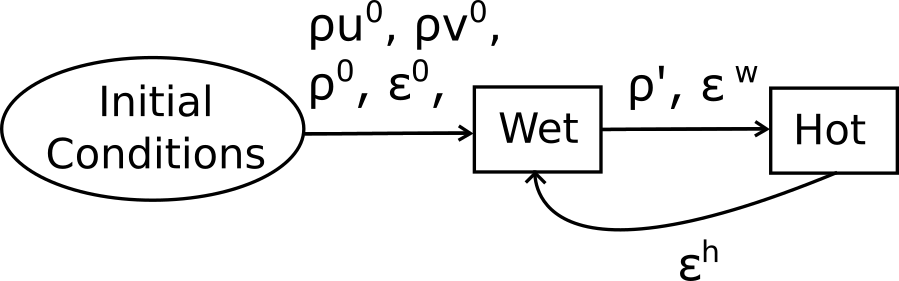
\includegraphics[width=1.0\linewidth]{hot-wet-flow}
\caption{The flow of our coupled Hot and Wet applications.}
\label{fig:hot-wet-flow}
\end{figure}

Figure \ref{fig:hot-wet-flow} demonstrates the current coupling, as well as the prospective coupling we plan to extend this work to accommodate. 

\section{Asynchronicity Among Packages}

Modern hardware presents a number of challenges and some important opportunities. The balance of different packages within a full application might allow new avenues for overlapping long communications or IO times, and even the potential for overlapping the compute of packages within the full application. We are interested to explore a number of these issues and expect that this could be a future direction for work but have not investigated that point in this research.

\section{Application Scaling}

As we are presenting two applications that have been developed from scratch, we provide some simple scaling studies to demonstrate that each application performs to an acceptable level. This data gives us some baseline for comparison as we consider the applications within a multi-algorithmic execution setting.

\begin{figure}
\centering
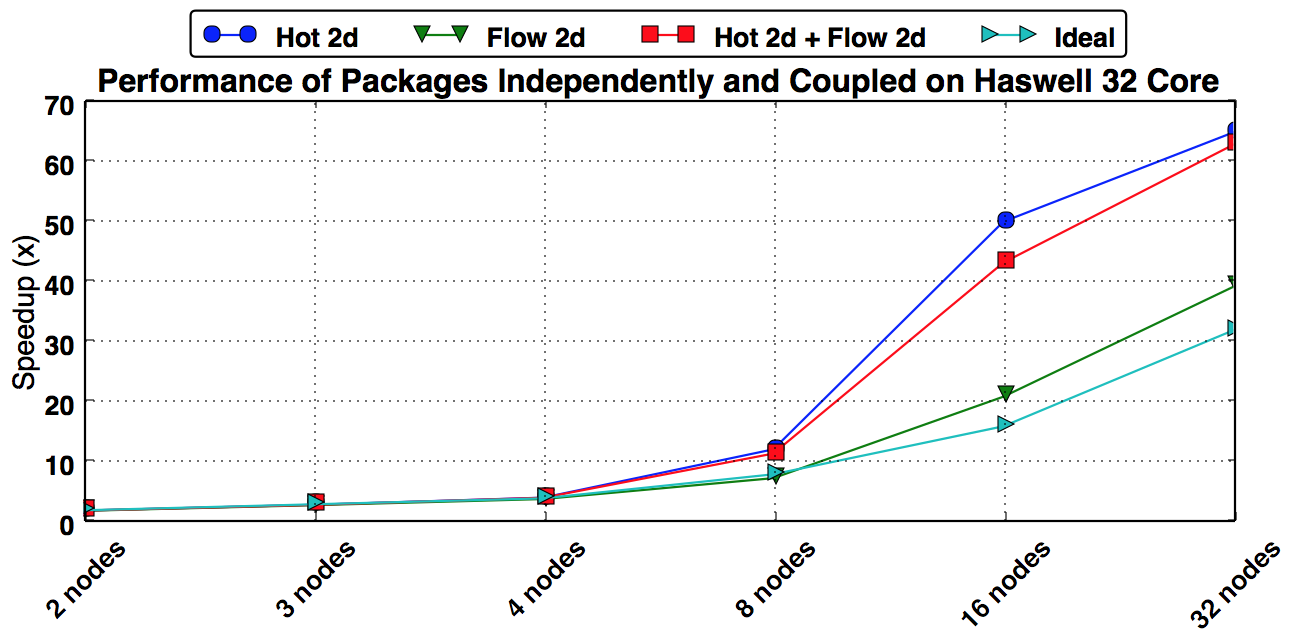
\includegraphics[height=6.2cm]{cpu_results}
\caption{}
\label{fig:example}
\end{figure}

\section{Patterns Inhibiting Performance for Multi-Package Applications}

Although both Hot and Wet combined together successfully, our research has uncovered a number of areas that we recognise will inhibit the performance of multi-package applications. In fact, it is possible to categorise those issues:

\begin{itemize}
  \item \textbf{Dynamic Meshes} - In the event that mesh data has to move between applications, there is significant potential.
  \item \textbf{Competing Decompositions} - It is possible that different packages within an application might require different decompositions for optimal performance.
  \item \textbf{Capacity Requirements} - As you increase the number of packages that are 
\end{itemize}

We hope that our future research can extend the results of this paper to begin to understand the issues we hypthesise here.

\section{Future Couplings}

We believe that it will be useful to extend this work to investigate the performance of diverse applications types, in particular we plan to develop new applications that cover the seven dwarves of parallel programming. There are many possible combinations that can occur within a multi-package applications depending on the requirements of the particular scientific question being solved. It is possible to consider many potential 

\begin{figure}
\centering
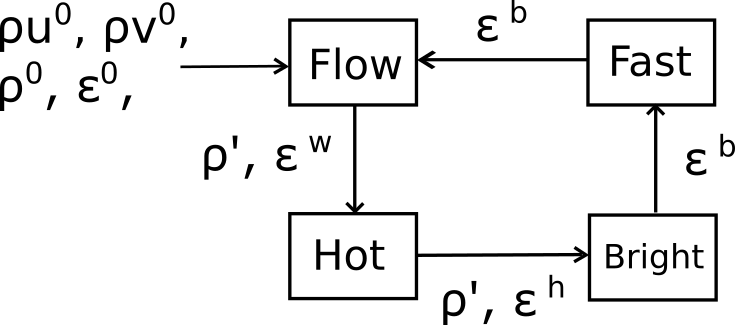
\includegraphics[width=1.0\linewidth]{all-four-flow}
\caption{The flow of a prospective multi-package application.}
\label{fig:multi-package-flow}
\end{figure}

\section{Future Work}

We further recognise that there are many requirements not handled by our existing applications, such as three-dimensional solves, multiple materials, and complex unstructured geometries. Each of these has a significant influence on the performance of individual algorithms, and likely introduces new issues for coupling packages together. As such it will be essential to consider new mini-apps that can proxy those particular features and consider their performance on new hardware.

\section{Related Work}

(SPEAK TO W ABOUT THIS SECTION, WHAT IS ACCEPTABLE TO BE TIED TO THIS PAPER)

\section{Conclusion}

\bibliographystyle{IEEEtran}
\bibliography{IEEEabrv,multi}

\end{document}

